\chapter{深度伪造的研究工具与检测手段的分类}
\label{chap:3}

本章节探讨深度伪造的研究工具与检测手段的分类,首先会根据 Thanh Thi Nguyen 等人 \cite{https://doi.org/10.48550/arxiv.1909.11573} 所进行的研究工作的简述,在他们的工作总结中将其工具分为两大类,也就是图像检测与人脸视频检测,并有着详细的整理,此外根据 Li XR 等人近期对深度伪造与检测的汇整工作\cite{2021496} 也有着详尽的说明,本作业除了针对究工具与检测手段等研究者们的近来工作将其汇整于此章。

\begin{figure}[htb]
\centering 
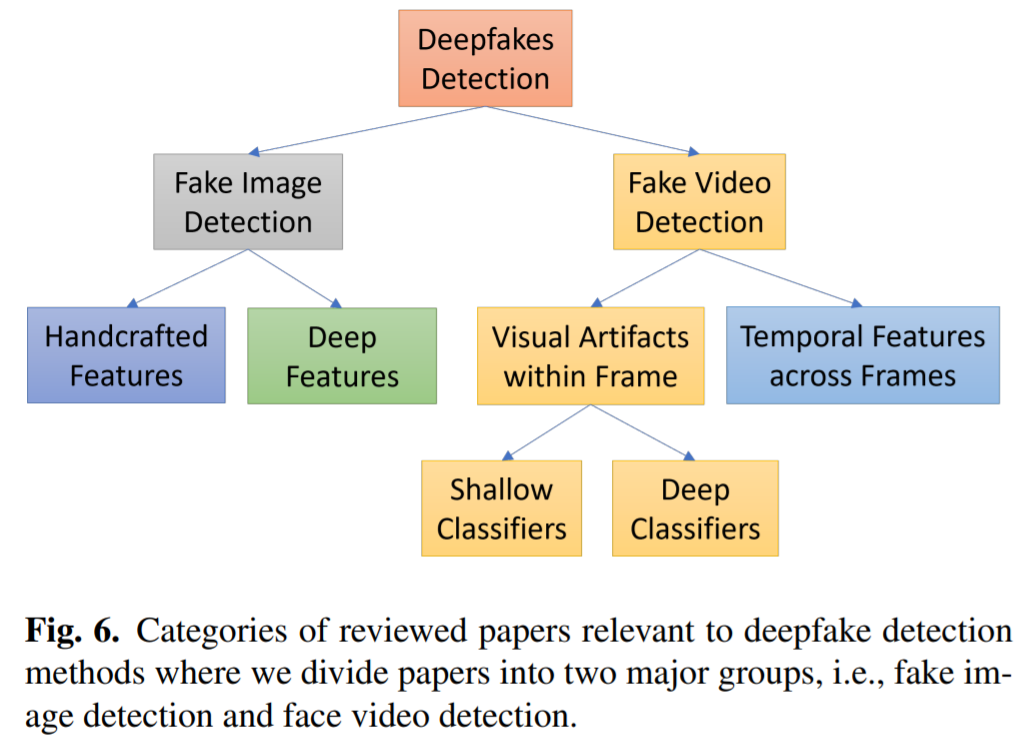
\includegraphics[width=0.90\textwidth]{img/ch3m1.png} 
\caption{从由 Thanh Thi Nguyen 等人 \cite{https://doi.org/10.48550/arxiv.1909.11573} 将深度伪造的伪造分为两大类}
\label{Test}
\end{figure}


\section{深度伪造的图像检测与人脸视频检测整理}

根据由 Thanh Thi Nguyen 等人 \cite{https://doi.org/10.48550/arxiv.1909.11573}的在深度伪造的工作中所整理的分类整理的过程中将其分为了图像检测与人脸视频检测。同时该工作也有将其深度伪造的检测手段进行总结,本作业根据原总结工作再汇整为深度伪造检测手段整理两表,两表之中总共有 24 种检测手段,这当中又因该工作所进行的分类,而分为三部分,其一为针对图像的检测,列于表二,共有 9 种手段,其二为影像的检测手段,其列于表一,共有 13 种手段,其三为图像检测与人脸视频检测皆可的检测,只有两种手段,并与表二图像检测并列。



%\begin{table}[ht]
%  \caption{test}
%  \label{Tab:bookRWCal}
%  \centering
%  \begin{tabular}{lp{3cm}p{3cm}p{3cm}}
%  \toprule
%  \textbf{著作类别} &\textbf{A级出版社} &\textbf{B级出版社}&\textbf{C级出版社}\\
%  \midrule
%  学术专著         &第一作者3分/万字,其他作者 2分/万字	&第一作者3分/万字,其他作者 2分/万字	&第一作者3分/万字,其他作者 2分/万字\\
%  \bottomrule
%  \end{tabular}
%\end{table}

\begin{table}[ht]
  \caption{深度伪造检测手段整理}
  \label{Tab:bookRWCal}
  \centering
  %\begin{tabular}{lp{3cm}p{2cm}p{2cm}}
  \begin{tabular}{p{3cm}p{3cm}p{3cm}p{3cm}}
  \toprule
  \textbf{方法} &\textbf{技術} &\textbf{检测种类}&\textbf{备注}\\
  \midrule
 Eye blinking & LRCN & Videos & Yuezun Li 等人\\
 Intra-frame and temporal inconsistencies & CNN and LSTM & Videos & David Guera 等人\\
 Using face warping artifacts & VGG16, ResNet models & Videos & Yuezun Li 等人\\
 MesoNet & CNN & Videos & Darius Afchar 等人\\
 Eye, teach and facial texture & Logistic regression and neural network(NN) & Videos & Falko Matern 等人\\
 Spatio-temporal features with RCN & RCN & Videos & Ekraam Sabir 等人\\
 Spatio-temporal features with LSTM & Convolutional bidirectional recurrent LSTM network & Videos & Akash Chintha 等人\\
 Analysis of PRNU & PRNU & Videos & Marissa Koopman 等人\\
 Phoneme-viseme mismatches & CNN & Videos & Shruti Agarwal 等人\\
 Using attributionbased confidence (ABC) metric & ResNet50 model, pre-trained on VGGFace2 & Videos & Steven Fernandes 等人\\
 Using appearance and behaviour & Rules based on facial and behavioural features & Videos &  Shruti Agarwal 等人\\
 FakeCatcher & CNN & Videos & Umur Aybars Ciftci 等人\\
 Emotion audiovisual affective cues & Siamese network & Videos & Trisha Mittal 等人\\
  \bottomrule
  \end{tabular}
\end{table}

\begin{table}[ht]
  \caption{深度伪造检测手段整理(续)}
  \label{Tab:bookRWCal}
  \centering
  %\begin{tabular}{lp{3cm}p{2cm}p{2cm}}
  \begin{tabular}{p{3cm}p{3cm}p{3cm}p{3cm}}
  \toprule
  \textbf{方法} &\textbf{技術} &\textbf{检测种类}&\textbf{备注}\\
  \midrule
 Head poses & SVM & Videos and Images & Xin Yang 等人\\
 Capsule-forensics & Capsule networks & Videos and Images & Huy H Nguyen 等人\\
 Preprocessing combined with deep network & DCGAN, WGAN-GP and PGGAN. & Images & Xinsheng Xuan 等人\\
 Analyzing convolutional traces & KNN, SVM, and linear discriminant analysis (LDA) & Images &  Luca Guarnera 等人\\
 Bag of words and shallow classifiers & SVM, RF, MLP & Images & Ying Zhang 等人\\
 Pairwise learning & CNN concatenated to CFFN & Images & Chih-Chung Hsu 等人\\
 Defenses against adversarial perturbations in deepfakes & VGG and ResNet & Images &  Apurva Gandhi 等人\\
 Face X-ray & CNN & Images & Chih-Chung Hsu 等人\\
 Using common artifacts of CNN-generated images & ResNet-50 pre-trained with ImageNet & Images & Sheng-Yu Wang 等人\\
 Using convolutional traces on GAN-based images & KNN, SVM, and LDA & Images & Luca Guarnera 等人\\
 Using deep features extracted by CNN & A new CNN model, namely SCnet & Images & Zhiqing Guo 等人\\
  \bottomrule
  \end{tabular}
\end{table}

\section{过往传统的检测手段}

过往的方式多为根据图像的特征来进行,其手段大多为信号的处理方式,且多数依赖某些特有的窜改证据,同时根据图像本身自有的频域特征与统计特征来进行分类,这些方式如噪音分析、设备指纹、光照、图像品质、处理复制移动、拼接、移除等问题,其实际工作比如 De Carvalho TJ 等人 \cite{de2013exposing},提出了一种伪造检测方法,该方法利用图像照明颜色的细微不一致,其方法是基于机器学习的,并且需要最少的用户交互。该技术适用于包含两个或更多人的图像,并且不需要专家交互来做出篡改决定,为了实现这一点,研究者将来自基于物理和统计的光源估计器的信息整合到类似材料的图像区域上。从这些光源估计中,该研究者提取基于纹理和边缘的特征,然后将其提供给机器学习方法以进行自动决策。使用 SVM 元融合分类器的分类性能是有希望的。它在由 200 张图像组成的新基准数据集上产生 86\% 的检测率,在从 Internet 收集的 50 张图像上产生 83\% 的检测率。

\begin{figure}[htb]
\centering 
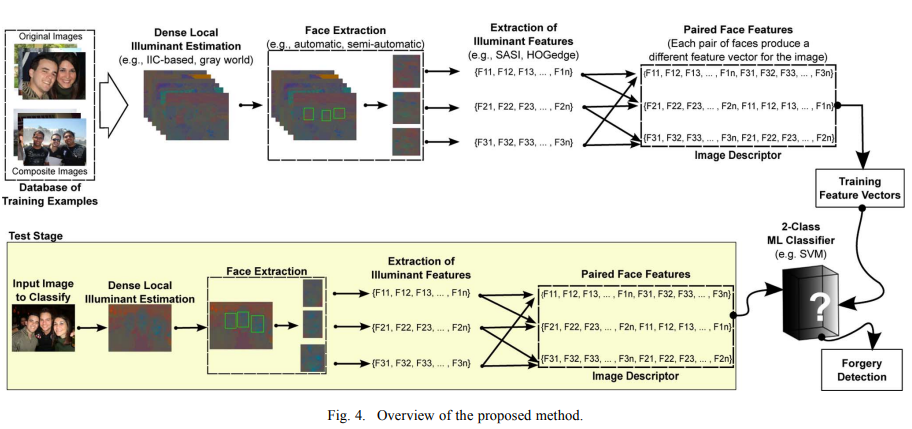
\includegraphics[width=0.90\textwidth]{img/ch3m2.png} 
\caption{De Carvalho TJ 等人 \cite{de2013exposing}}
\label{Test}
\end{figure}

另外  Amerini I 等人 \cite{amerini2011sift} 则探究图像是否被伪造的检测问题;特别是,图像的一个区域被复制然后粘贴到另一个区域用以创建复制或取消一些尴尬的东西的情况。通常来说为了使图像补丁适应新的上下文,需要进行几何变换。为了检测这种修改,提出了一种基于尺度不变特征变换(SIFT)的新方法。这种方法使研究者既可以了解是否发生了复制移动攻击,还可以恢复用于执行克隆的几何变换。广泛的实验结果证实了该技术能够精确地个体化改变区域,此外,还能够以高可靠性估计几何变换参数。该方法还处理多重复制。

同理可推,其深度伪造的影像的本质,实质上也是一连串的图像伪造的工作合成后所完成的结果,也因为如此,此类检测方式与手段就能使用到深度伪造的检测工作上。而 Lukáš J \cite{lukavs2006detecting} 等人提出了一种检测数字图像中的伪造品的新方法,其方法基于检测图像中各个区域中相机模式噪声的存在,这是成像传感器的独特随机特性。而伪造区域被确定为缺少图案噪声的区域。噪声的存在是使用相关性确定的,如在扩频水印的检测中。研究者们提出了两种方法在第一个中,用户选择一个区域进行完整性验证。第二种方法试图在不假设任何先验知识的情况下自动确定伪造区域。这些方法在真实伪造的例子和非伪造图像上都进行了测试,其研究者还研究了应用于伪造图像的进一步图像处理,例如有损压缩或过滤,如何影响验证图像完整性的能力。

\begin{figure}[htb]
\centering 
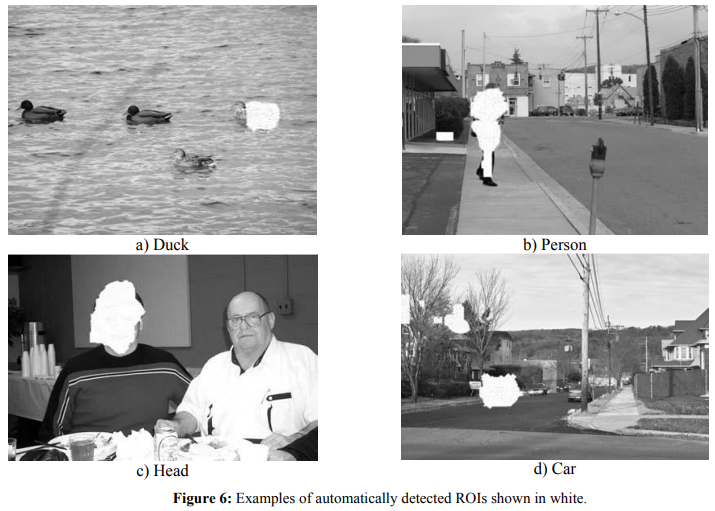
\includegraphics[width=0.90\textwidth]{img/ch3m3.png} 
\caption{Lukáš J 等人 \cite{lukavs2006detecting}}
\label{Test}
\end{figure}

Chierchia G 等人 \cite{chierchia2011prnu} 引入了光响应非均匀性 (PRNU) 作为检测图像伪造的强大工具,尽管它在许多情况下都有效,但所提出的方法无法检测到小的操作。在这项工作中,研究者基于图像的初步分割提出了中描述的检测算法的修改版本,这保证了对小尺寸加法伪造品的更好检测性能。而 Fridrich J 等人 \cite{fridrich2012rich} 则提出一种新的通用策略,用于为数字图像构建隐写检测器,该过程首先组装一个丰富的噪声分量模型,作为由使用线性和非线性高通滤波器获得的量化图像噪声残差的相邻样本的联合分布形成的许多不同子模型的联合。与以前的方法相比,研究者使模型组装成为训练过程的一部分,该过程由从相应的覆盖和隐秘源中抽取的样本驱动。集成分类器用于组装模型以及最终的隐写分析器,因为它们的计算复杂度低并且能够有效地处理高维特征空间和大型训练集。该研究在三种隐写算法上演示了所提出的框架,这些演算法旨在隐藏空间域中表示的图像中的消息:HUGO、Luo 的边缘自适应算法和优化编码的三元 ±1 嵌入。对于每种算法,研究者应用一种简单的子模型选择技术来提高每个模型维度的检测精度,并展示检测如何随着丰富模型的复杂性增加而饱和。通过观察不同子模型如何参与检测之间的差异,揭示了嵌入和检测之间有趣的相互作用。围绕丰富的图像模型构建的隐写分析与集成分类器相结合,是为广泛的隐写方案自动化隐写分析的一个有前途的方向。另外 Wang W 等人 \cite{wang2014exploring} 则专注于局部图像篡改检测。对于 JPEG 图像,其 DCT 系数的概率分布会受到篡改操作的干扰,篡改区域和未改动区域分布不同,是定位篡改的重要线索。基于未量化的ac DCT系数的拉普拉斯分布假设,可以估计这两个分布以及被篡改区域的大小,从而得到每个DCT块被篡改的概率,当研究者考虑常见篡改区域的先验知识时,可以获得更准确的定位结果,其研究者还设计了三种可以区分真实篡改区域和虚假区域的特征,以减少误报。对于以无损压缩格式保存的篡改图像,而研究者还提出了一种专门的方法,该方法利用高频DCT系数的量化噪声来提高篡改定位性能。在大规模数据库上的大量实验证明了该研究提出的方法的有效性,并证明其方法适用于定位不同尺度的篡改区域。

此外還對 JPEG 压缩的图像中添加噪声來進行檢測的研究,比如 Nataraj L 等人 \cite{nataraj2009adding} 认为影响大多数图像大小调整检测算法的一个常见问题是它们容易受到 JPEG 压缩的影响,这是因为 JPEG 引入了周期性伪影,因为它适用于 8×8 块。其研究者提出了一种新颖但反直觉的技术,通过添加高斯噪声来“去噪”JPEG 图像。其研究者将适量的高斯噪声添加到调整大小和 JPEG 压缩的图像中,以便抑制由于 JPEG 压缩而导致的周期性,而由于调整大小而导致的周期性得以保留,受控的高斯噪声添加比中值滤波和基于加权平均的滤波更有效地抑制 JPEG 引起的周期性。

\begin{figure}[htb]
\centering 
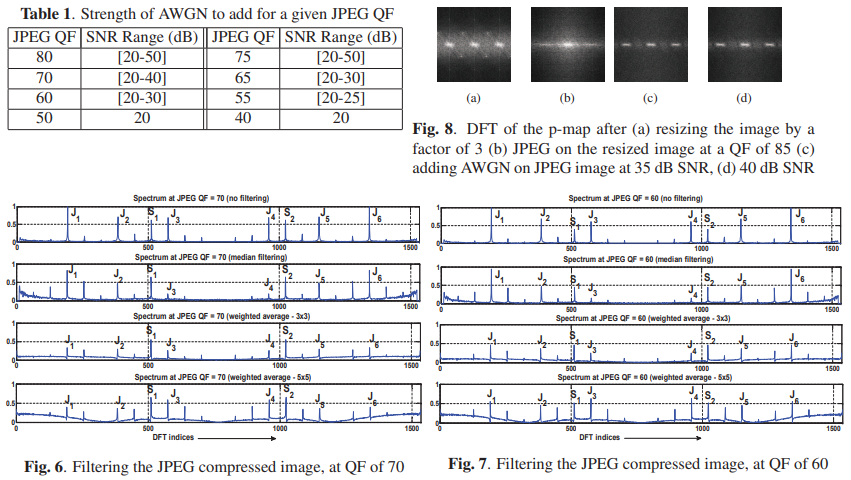
\includegraphics[width=0.90\textwidth]{img/ch3m4.png} 
\caption{Nataraj L 等人 \cite{nataraj2009adding}}
\label{Test}
\end{figure}

同时 Bianchi T 等人 \cite{bianchi2011improved} 提出了一种统计测试来区分 JPEG 图像中的原始区域和伪造区域,假设前者是双重压缩的,而后者是单次压缩的。提出了单压缩和双压缩区域 DCT 系数的新概率模型,以及双压缩情况下估计主量化因子的可靠方法,基于这样的模型,推导出每个 DCT 块被伪造的概率,其实验结果证明了相对于先前提出的方法更好的区分行为。

另外有些研究者则运用局部噪音方差分析的特性来拼接痕迹 Pan X 等人 \cite{pan2012exposing} 所提出的研究是基于来自不同来源的图像往往具有由传感器或后处理步骤引入的不同数量的噪声,研究者描述了一种通过检测局部噪声方差的不一致性来暴露图像拼接的有效方法,其方法基于以下观察估计局部噪声方差:带通滤波域中自然图像的峰度值倾向于集中在一个恒定值附近,并通过使用积分图像来加速。最后基于通过图像拼接生成的几组伪造图像证明了我们方法的有效性和鲁棒性。

而 Ferrara P \cite{6210378} 等人则是运用 色彩过滤矩阵 (Color Filter Array; CFA) 模型来找出修改过的地方,该研究提出了一种能够区分数码相机捕获的图像中的原始区域和伪造区域的取证工具,研究者假设图像是使用滤色器阵列获取的,并且由于去马赛克算法,篡改会消除伪影,其所提出的方法是基于一个新的特征来测量局部水平的去马赛克伪影的存在,以及一个新的统计模型,允许推导出每个 2 × 2 图像块的篡改概率,而无需先验地知道伪造的位置。最后在配备不同去马赛克算法的不同相机上的实验结果证明了理论模型的有效性和方案的有效性。

\begin{figure}[htb]
\centering 
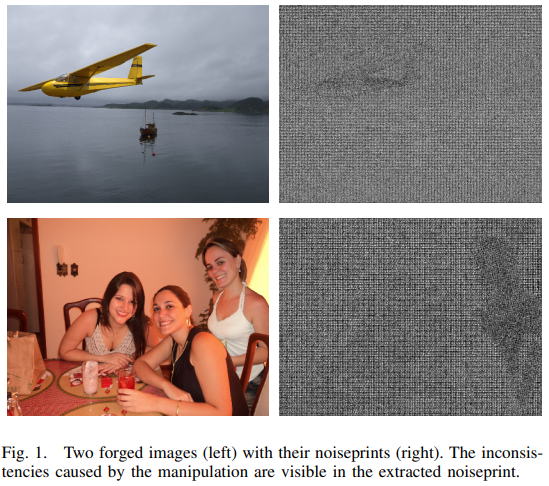
\includegraphics[width=0.90\textwidth]{img/ch3m5.png} 
\caption{Cozzolino D 等人 \cite{cozzolino2019noiseprint}}
\label{Test}
\end{figure}

由于近年来人工智能领域的进步,当中的机器学习下的深度学习方法逐渐导入检测手段中,其卷积神经网络、生成对抗网路与 Transformer 等模型,在该领域的应对皆超越了过往的纪录,而且成功率大大的提升,相较上述过往图像特征的检测方式,前者的鲁棒性更好。Cozzolino D 等人 \cite{cozzolino2019noiseprint} 则认为数字图像的取证分析在很大程度上依赖于在获取的图像上留下的相机内和相机外过程的痕迹,这样的痕迹代表了一种相机指纹,若能够恢复它们,通过抑制高级场景内容和其他干扰,可以轻松完成多项取证任务。一个值得注意的例子是 PRNU 模式,它可以被视为设备指纹,在多媒体取证中受到了极大的关注。该研究提出了一种提取相机模型指纹的方法,称为噪声指纹,其中场景内容在很大程度上被抑制,与模型相关的伪影得到增强。这是通过连体网络获得的,该网络使用来自相同(标签 +1)或不同(标签 -1)相机的成对图像块进行训练。尽管噪声印记可用于多种取证任务,但这里我们专注于图像伪造定位,而在广泛使用的几个数据集上的实验表明,基于噪声印记的方法可以提供最先进的性能。Zhou P 等人 \cite{zhou2018learning}认为图像操作检测不同于传统的语义对象检测,因为它更关注篡改伪影而不是图像内容,这表明需要学习更丰富的特征,研究者提出了一个双流 Faster R-CNN 网络并对其进行端到端训练,以检测给定操纵图像的篡改区域。两个流之一是 RGB 流,其目的是从 RGB 图像输入中提取特征,以发现篡改伪影,如强对比度差异、不自然的篡改边界等。另一种是噪声流,它利用从隐写分析丰富的模型过滤层中提取的噪声特征来发现真实区域和篡改区域之间的噪声不一致。然后,研究者通过双线性池化层融合来自两个流的特征,以进一步结合这两种模式的空间共现。对四个标准图像处理数据集的实验表明,其双流框架优于每个单独的流,并且与具有调整大小和压缩鲁棒性的替代方法相比,还实现了最先进的性能。

Rao Y 等人 \cite{rao2016deep} 提出了一种基于深度学习技术的新图像伪造检测方法,该方法利用卷积神经网络 (CNN) 从输入的 RGB 彩色图像中自动学习层次表示,所提出的 CNN 专为图像拼接和复制移动检测应用而设计,其网络第一层的权重不是随机策略,而是使用空间丰富模型 (SRM) 中残差图计算中使用的基本高通滤波器集进行初始化,作为正则化器,可以有效地抑制图像内容并捕获由篡改操作引入的细微伪影,将预训练的 CNN 作为补丁描述符从测试图像中提取密集特征,然后探索特征融合技术以获得 SVM 分类的最终判别特征。在几个公共数据集上的实验结果表明,所提出的基于 CNN 的模型优于一些最先进的方法。Liu B 等人 \cite{liu2018deep} 提出了一种新颖的深度融合网络,通过跟踪其边界来定位篡改区域,首先训练了一组称为 Base-Net 的深度卷积神经网络来分别响应某种类型的拼接伪造。然后,选择 Base-Net 的一些层并组合为深度融合神经网络(Fusion-Net),经过极少量的图片微调后,Fusion-Net 能够辨别图像块是否是从不同来源合成的。在基准数据集上的实验表明,该研究方法在各种情况下都是有效的,并且优于最先进的方法。Huh M 等人  \cite{huh2018fighting} 认为照片编辑和操作工具的进步使得创建假图像变得更加容易,突出了对更好的视觉取证算法的需求,然而,由于缺乏被操纵的视觉内容的良好数据集,学习从标记的训练数据中检测操纵是困难的,该研究介绍了一种自我监督方法,用于学习仅使用未标记数据来检测视觉操作。给定大量带有自动记录的 EXIF 元数据的真实照片,研究者训练一个模型来确定图像是否是自洽的——也就是说,它的内容是否可以由单个成像管道产生。研究者将这种自我监督学习方法应用于定位拼接图像内容的任务。其取证模型在许多基准上都取得了最先进的结果,尽管在没有实际操作示例的情况下进行了训练,也没有对特定的检测线索进行建模。除了手工制作的基准之外,研究者还展示了在 Reddit 和 The Onion 上发现假货以及检测计算机生成的拼接的有希望的结果。Cun X 等人 \cite{cun2018image} 解决了图像拼接定位的问题:给定一张输入图像,定位从另一张图像中剪下的拼接区域,并将其制定为分类任务,但关键的是,我们不是通过局部补丁对拼接区域进行分类,而是利用整个图像和局部补丁的特征来对补丁进行分类。而研究者们称这种结构为 Semi-Global Network,其方法利用了拼接区域不仅应与局部特征(拼接边缘)高度相关,还应与整个图像的全局特征(语义信息、照明等)高度相关的观察结果。此外,该研究首先将全连接条件随机场作为图像拼接中的后处理技术,以提高输入图像和网络输出之间的一致性。

Cozzolino D 等人 \cite{cozzolino2017recasting} 基于图像噪声残差的局部描述符已被证明对于许多取证应用非常有效,例如伪造检测和定位,尽管如此,在计算机视觉领域取得可喜成果的推动下,研究界的重点现在正在转向深度学习。该研究展示了一类基于残差的描述符实际上可以被视为一个简单的约束卷积神经网络(CNN)。通过放松约束,并在相对较小的训练集上微调网络,其成果相对于传统检测器获得了显著的性能提升。

\begin{figure}[htb]
\centering 
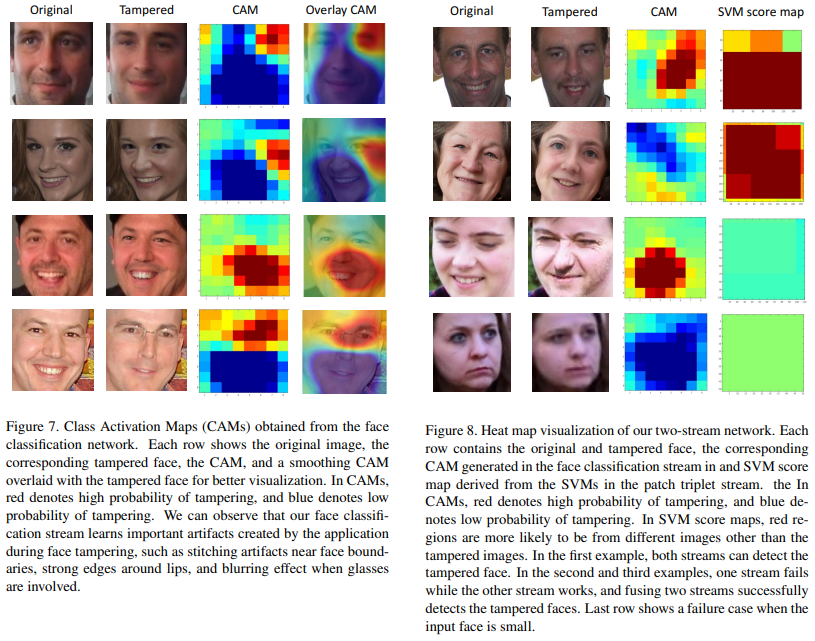
\includegraphics[width=0.90\textwidth]{img/ch3m6.png} 
\caption{Zhou P 等人 \cite{zhou2017two}}
\label{Test}
\end{figure}

Chen C 等人 \cite{chen2018focus} 认为随着通过社交媒体渠道传播的错误信息的兴起,以及图像处理工具的自动化和真实性的提高,图像取证成为一个越来越重要的问题,经典的图像取证方法利用低级线索,例如元数据、传感器噪声指纹等,当图像在上传到 Facebook 等时重新编码时很容易被愚弄。这需要使用更高级别的物理和语义线索,这些线索曾经在野外难以可靠地估计,但由于计算机视觉的能力越来越强,它们变得更加有效。特别是,该研究的检测由图像的人工模糊引入的操作,这会在图像强度和各种线索之间产生不一致的光度关系。在一个新的模糊操作数据集中,研究者在最具挑战性的情况下实现了 98\% 的准确率,其中模糊在几何上是正确的并且与场景的一致 物理安排。这种操作现在很容易生成,例如,通过具有硬件来测量深度的智能手机相机,例如。 iPhone7Plus 的“人像模式”。最后还在挑战数据集上展示了良好的性能,该数据集评估了代表“野外”条件的图像中更广泛的操作。

Zhou P 等人 \cite{zhou2017two} 则根据 Szegedy C 等人 \cite{szegedy2015going}所提出的基础上,做出了一种用于人脸篡改检测的双流网络,其训练 GoogLeNet 以检测人脸分类流中的篡改伪影,并训练基于补丁的三元组网络以利用捕获局部噪声残差和相机特征的特征作为第二个流。此外,研究者使用两个不同的在线人脸交换应用程序来创建一个新的数据集,该数据集由 2010 个篡改图像组成,每个图像都包含一个被篡改的人脸。最后在新收集的数据集上评估提出的双流网络。实验结果证明了其方法的有效性。

\section{人类的生理特征的检测手段}

深度伪造的影像往往会忽视人类正常活动的生理特征,因而无法在整体的状况下与真实人类的行动与反应一致,所以根据人类的生理信号特征也进入了研究者们关注的部分。 Yang X 等人 \cite{yang2019exposing} 所提出的方法是基于观察到 DeepFakes 是通过将合成的人脸区域拼接到原始图像中来创建的,并且在这样做的过程中,当从人脸图像估计 3D 头部姿势时可以发现错误。研究者进行实验来证明这种现象,并进一步开发基于这种线索的分类方法。使用基于此线索的特征,使用一组真实面部图像和 DeepFakes 评估 SVM 分类器。同样也是 Yang X 等人 \cite{yang2019exposing} 发现生成对抗网络(GAN)最近导致了高度逼真的图像合成结果。在这项工作中,研究者描述了一种使用面部标志点的位置来展示 GAN 合成图像的新方法。其方法是基于观察到,由于缺乏全局约束,GAN 模型生成的面部部件配置与真实面部不同。研究者进行了演示这种现象的实验,并表明使用面部标志点的位置训练的 SVM 分类器足以为 GAN 合成的面部实现良好的分类性能。

\begin{figure}[htb]
\centering 
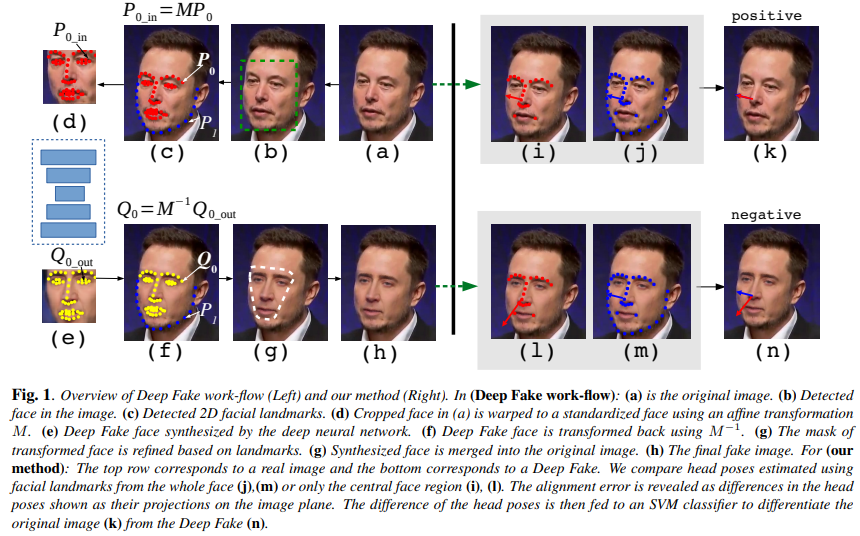
\includegraphics[width=0.90\textwidth]{img/ch3m7.png} 
\caption{Yang X 等人 \cite{yang2019exposing}}
\label{Test}
\end{figure}

另外 Li Y 等人 \cite{liy2018exposingaicreated} 认为深度生成网络的新发展显著提高了生成逼真的假人脸视频的质量和效率。在这项工作中,研究者描述了一种新方法来暴露由深度神经网络模型生成的假人脸视频,其方法基于检测视频中的眨眼,这是一种生理信号,在合成的假视频中没有很好地呈现。该方法在眨眼检测数据集的基准上进行了评估,并在检测使用基于 DNN 的软件 DeepFake 生成的视频方面表现出良好的性能。

而 Ciftci UA 等人 \cite{ciftci2020fakecatcher} 提出了一种检测肖像视频中合成内容的新方法,作为针对深度伪造威胁的预防性解决方案。换句话说,该研究引入了一个深度伪造检测器,研究观察到,盲目地利用深度学习的检测器无法有效捕捉虚假内容,因为生成模型会产生非常逼真的结果。其研究者的关键断言是,隐藏在肖像视频中的生物信号可以用作真实性的隐含描述符,因为它们既不会在空间上也不会在时间上保留在虚假内容中。为了证明和利用这一断言,该研究首先对成对分离问题进行了几次信号转换,达到了 99.39\% 的准确率。其次,通过分析建议的信号转换和相应的特征集,利用这些发现为虚假内容制定通用分类器。第三,生成新的信号图并使用 CNN 来改进我们用于检测合成内容的传统分类器。最后,发布了一个“在野外”的假肖像视频数据集,而后在评估过程中收集了该数据集。研究在几个数据集上评估 FakeCatcher,分别在人脸取证、人脸取证++、CelebDF 和研究本身新的 Deep Fakes 数据集上获得 96\%、94.65\%、91.50\% 和 91.07\% 的准确率。该研究还分析了来自不同面部区域的信号,在图像失真下,具有不同的片段持续时间,来自不同的生成器,针对看不见的数据集,以及在几种降维技术下。

同时 Fernandes S 等人 \cite{fernandes2019predicting} 获得了原始视频的心率并训练了最先进的神经常微分方程 (Neural-ODE) 模型。然后,研究者使用商业软件制作了 deepfake 视频,其十个原始视频获得的平均损失为 0.010927,十个捐赠视频为 0.010041,经过训练的 Neural-ODE 能够预测我们使用商业软件生成的 10 个 deepfake 视频和 deepfakeTIMI 数据库的 320 个 deepfake 视频的 heart rate,据该研究者所知,这是首次尝试在原始视频上训练 Neural-ODE 来预测假视频的 heart rate。


\section{图像伪造后留下痕迹的检测手段}

\begin{figure}[htb]
\centering 
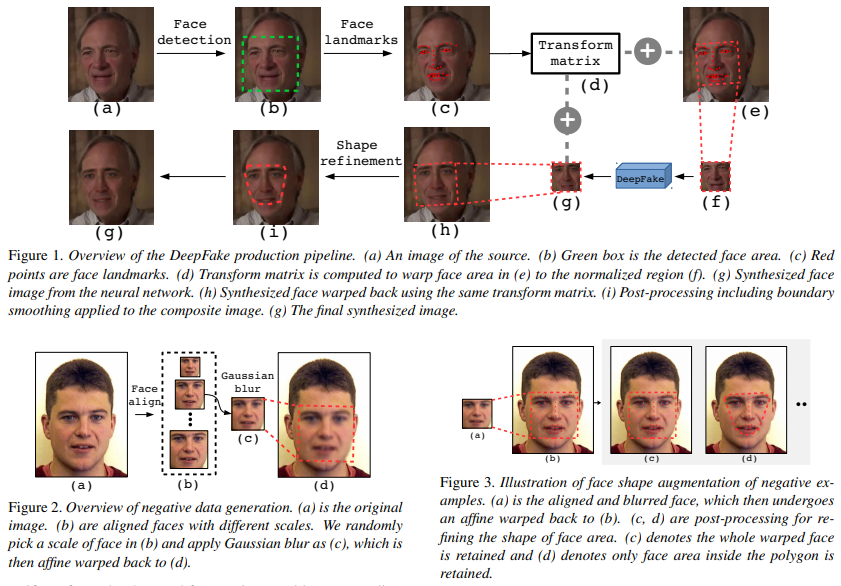
\includegraphics[width=0.90\textwidth]{img/ch3m8.png} 
\caption{ Li Y 等人 \cite{li2018exposing} }
\label{Test}
\end{figure}

其深度伪造的成果受限于过往深度学习的技术发展,用此技术所生成的人类脸部替换或者是伪造的细节皆没有很理想,因此不少研究者为此投入这个部分,而 Li Y 等人 \cite{li2018exposing} 描述了一种新的基于深度学习的方法,可以有效地将 AI 生成的假视频(以下称为 {\em DeepFake} 视频)与真实视频区分开来。其方法基于当前 DeepFake 算法只能生成分辨率有限的图像的观察结果,这些图像需要进一步变形以匹配源视频中的原始人脸,这种变换在生成的 DeepFake 视频中留下了独特的伪影,我们证明它们可以被卷积神经网络 (CNN) 有效地捕获,与以前使用大量真实和 DeepFake 生成的图像来训练 CNN 分类器的方法相比,该方法不需要 DeepFake 生成的图像作为负训练示例,因为研究将仿射面部扭曲中的伪影作为区分真假的显著特征图片。其研究方法的优点有两个:(1)可以直接对图像使用简单的图像处理操作来模拟这种伪影,使其成为反例。由于训练 DeepFake 模型生成负样本既费时又需要资源,因此该研究的方法在训练数据收集方面节省了大量时间和资源; (2) 由于此类伪影普遍存在于来自不同来源的 DeepFake 视频中,因此该研究的方法与其他方法相比更加稳健,研究的方法在两组 DeepFake 视频数据集上进行了评估,以了解其在实践中的有效性。

最后 Li Y 等人 \cite{li2018exposing} 则是运用了 He K 等人 \cite{he2016deep}所做的一个残差学习框架,以简化比以前使用的网络更深的网络的训练,该研究明确地将层重新定义为参考层输入的学习残差函数,而不是学习未参考的函数。其提供了全面的经验证据,表明这些残差网络更容易优化,并且可以从显著增加的深度中获得准确性。在 ImageNet 数据集上,研究者评估深度高达 152 层的残差网络——比 VGG 网络深 8 倍,但仍然具有较低的复杂度,这些残差网络的集合在 ImageNet 测试集上实现了 3.57\% 的误差。该结果在 ILSVRC 2015 分类任务中获得第一名。我们还对具有 100 层和 1000 层的 CIFAR-10 进行了分析。表示的深度对于许多视觉识别任务至关重要,其研究在 COCO 对象检测数据集上获得了 28\% 的相对改进,深度残差网络是该研究提交 ILSVRC 和 COCO 2015 比赛的基础,研究者还在 ImageNet 检测、ImageNet 定位、COCO 检测和 COCO 分割任务中获得了第一名,也就是所谓的 ResNet 框架。

另外 Matern F 等人 \cite{matern2019exploiting} 回顾了当前的面部编辑方法和来自其处理管道的几个特征工件。其研究还表明,相对简单的视觉伪影在暴露此类操作方面已经非常有效,包括 Deepfakes 和 Face2Face 的成果。而该研究团队所用的辨别手段如下 :

\begin{itemize}
\item [-] 整体不一致性 : 其伪造手段所生成的人类脸部会有不协调这状况,比如左右眼珠、脸部、鼻子在颜色上不一致。
\item [-] 光影的不一致性 : 光线的照射往往都会被伪造的模型给忽略掉。
\item [-] 几何的不一致 : 细节上的牙齿、眼睛得缺失,又或者只有生成部分。
\end{itemize}

\section{ GAN 模型所产生的检测手段}


\section{图片的深度学习之检测手段}


\section{影像的深度学习之检测手段}















